\documentclass[10pt]{article}
\usepackage[utf8]{inputenc}
\usepackage{empheq}
\usepackage[inline, shortlabels]{enumitem}
\usepackage{gensymb}
\usepackage{multicol}
\setlength{\parskip}{0.5cm plus4mm minus3mm}
\setlength{\parindent}{0pt}
\usepackage{amsmath}
\usepackage{upgreek}
\usepackage[nobreak=true]{mdframed}
\usepackage[margin=0.6in]{geometry}
 \geometry{
 left=8mm,
 bottom=20mm
 }
\usepackage{changepage}
\usepackage{amssymb}
\usepackage{titlesec}
\usepackage{listings}
\usepackage{MnSymbol}
\usepackage{chngcntr}
\usepackage{graphicx}

\usepackage{cs170}


\newcommand{\norm}[1]{\lvert #1 \rvert}
\newcommand{\Est}[1]{\hat{#1}}
\newcommand{\argmax}{\operatornamewithlimits{argmax}}

\begin{document}
\date{}
\title{\vspace{-5ex} \dunhd{CS188: Artificial Intelligence Notes} \vspace{-5ex}}
\maketitle
\begin{multicols}{2}
\section{Search and Planning}
\begin{enumerate}
    \subsection{Search Problems} 
    \begin{enumerate}
         \item \textbf{Agents}
         \begin{enumerate}
             \item A \textbf{rational agent} is an entity that has goals or preferences and performs a series of actions that yield the best/optimal expected outcome given these goals.
             \item A \textbf{reflex agent} simply selects an action based solely on the current state of the world.
             \item A \textbf{planning agent} maintains a model of the world and uses this model to simulate performing various actions before selecting the best one.
         \end{enumerate} 
         
         \item A \textbf{world state} contains all information about a given state, whereas a \textbf{search state} contains only the information about the world that’s necessary for planning. A \textbf{Search problem} is defined by four things:
         \begin{enumerate}
             \item \textbf{State space:} The set of all possible states in a given world.
             \item \textbf{Successor function:} A function that takes in a state and an action and computes the cost of that action as well as the successor state.
             \item \textbf{Start state:} The state in which an agent exists initially.
             \item \textbf{Goal test:} Boolean-valued function for if a state is the goal state.
         \end{enumerate}
         
         \item \textbf{State Space size:} Determine the state representation. Then use the fundamental counting principle (multiply the number of different values each variable object take on). For example, with an $M \times N$ grid:
         \begin{itemize}
             \item For state representation (direction, $x$, $y$, speed), the size is $4MN(V_{max}+1)$. 
             \item For state representation ($x$, $y$, food pellet grid), the size is $MN2^{MN}$. 
         \end{itemize}
         
         \item
         A \textbf{state space graph} is constructed with nodes representing states, with directed edges to its successors. Each state appears exactly once. \textbf{Search trees}, on the other hand, have no restriction on the number of times a state appears. 
         
         \item \textbf{Search Algorithms} \\
         The general algorithm for graph search is as follows:
         \begin{align*}
             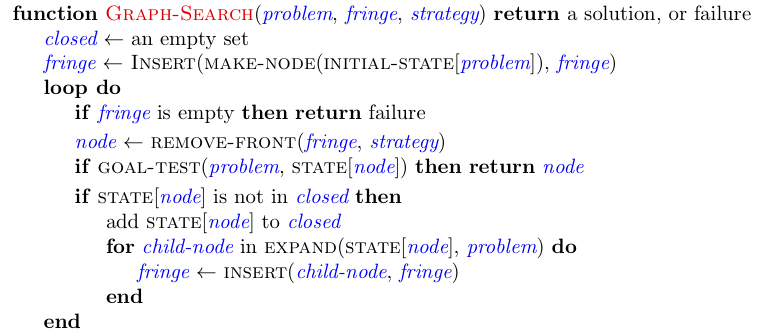
\includegraphics[scale=0.65]{graph_search.png}
         \end{align*}
         Note that tree search is identical except that it lacks a closed set and does not check if a node has been visited. \\ Also, a more memory efficient variant checks if a node is in the closed set before adding to the fringe.
         \begin{enumerate}
             \item \textbf{Complete:} The algorithm is guaranteed to find a solution if one exists.
             \item \textbf{Optimal:} The algorithm returns the least cost path to the goal.
             \item Let $b$ be the branching factor of the search tree (the number of states the successor function returns) and $m$ be the maximum depth of the search tree.
         \end{enumerate}
         
         \item \textbf{Depth First Search}
         \begin{enumerate}
             \item The fringe is implemented as a stack. 
             \item Only Graph-Search DFS is \textit{complete} (could get stuck in cycles in Tree Search). Obviously not optimal.
             \item Time complexity is $O(b^m)$. Space complexity is $O(bm)$.
         \end{enumerate}
         
         \item \textbf{Breadth First Search}
         \begin{enumerate}
             \item The fringe is implemented as a queue. 
             \item BFS is always \textit{complete}. Optimality guaranteed only if all edge weights are equal. 
             \item Time and space complexity is $O(b^s)$, where $s$ is the depth of the solution.
         \end{enumerate}
         
         \item \textbf{Uniform Cost Search (Dijkstra)}
         \begin{enumerate}
             \item The fringe is implemented as a priority queue, ordered by lowest cumulative distance traveled (\textit{computed backward cost}). 
             \item A more memory efficient variant updates the priority of a node on the fringe rather than adding another.
             \item UCS is complete and optimal.
             \item Let $C^*$ be the cost of the optimal path, and $\epsilon$ be the minimal edge weight between any two nodes in the state space graph. Then an upper bound on time and space complexity is $O(b^{C^* / \epsilon})$.
         \end{enumerate}
         
         \item \textbf{Greedy Search}
         \begin{enumerate}
             \item The fringe is implemented as a priority queue, ordered by lowest hueristic value.
             \item Not complete nor optimal.
         \end{enumerate}
         
         \item \textbf{A*}
         \begin{enumerate}
             \item The fringe is implemented as a priority queue, ordered by lowest computed backward cost \textit{plus} estimated forward cost (a heuristic).
             \item Both complete and optimal, given an appropriate heuristic (see below).
         \end{enumerate}
         
         \item \textbf{Heuristics}
         \begin{enumerate}
             \item A heuristic is a function $h(n)$ that takes in a state and returns a numeric estimate of the cost to the goal state. They are typically solutions to relaxed problems (ex: Manhattan distance, Euclidean distance).
             \item A heuristic is \textbf{admissible} if the value returned by the heuristic is neither negative nor greater than the true cost of reaching the goal from the given state.
             \item A heuristic is \textbf{consistent} if for all edges $A \rightarrow B$, $h(A) - h(B) \leq$ cost($A,B$). Consistency ensures that the first time a node is expanded, the cost to that state is optimal. 
             \item Any valid heuristic must have that $h(G)=0$.
             \item Consistency \textit{implies} admissibility.
             \item A* Tree search is guaranteed complete and optimal for any \textit{admissible} heuristic. A* graph search is guaranteed complete and optimal for any \textit{consistent} heuristic. Note that a simple fix for admissible but inconsistent heuristics is to allow a state to be expanded again if the cost to that state is lower than what it was last time it was expanded.

         \end{enumerate}
    \end{enumerate}
    
    \subsection{Constraint Satisfaction Problems} 
    Before, the path to the goal was most important. Now, only the goal itself is important. 
    \begin{enumerate}
        \item \textbf{CSP}s are a special subset of search problems. A state is defined by assignments to \textbf{variables} $X_i$. The set of values a variable $X_i$ can take on is the \textbf{domain} $D$. (We will only consider discrete variables with finite domains). The goal test is a set of constraints specifying allowable combinations of values for subsets of variables.
        \item A \textbf{unary} constraint is a constraint on a single variable (e.g., $X \geq 2$) while a \textbf{binary} constraint relates two variables (e.g., $X \geq Y$). In a binary constraint graph, each node is a variable and each edge is a constraint relating two variables. A non-binary CSP has constraints relating multiple variables (e.g., the standard constraints for Sudoku).
        \item \textbf{Backtracking Search} is DFS with two extra features:
        \begin{enumerate}
            \item Variables are ordered.
            \item Consider only values which do not conflict with previous constraints; incremental goal test.
        \end{enumerate}
        \begin{align*}
            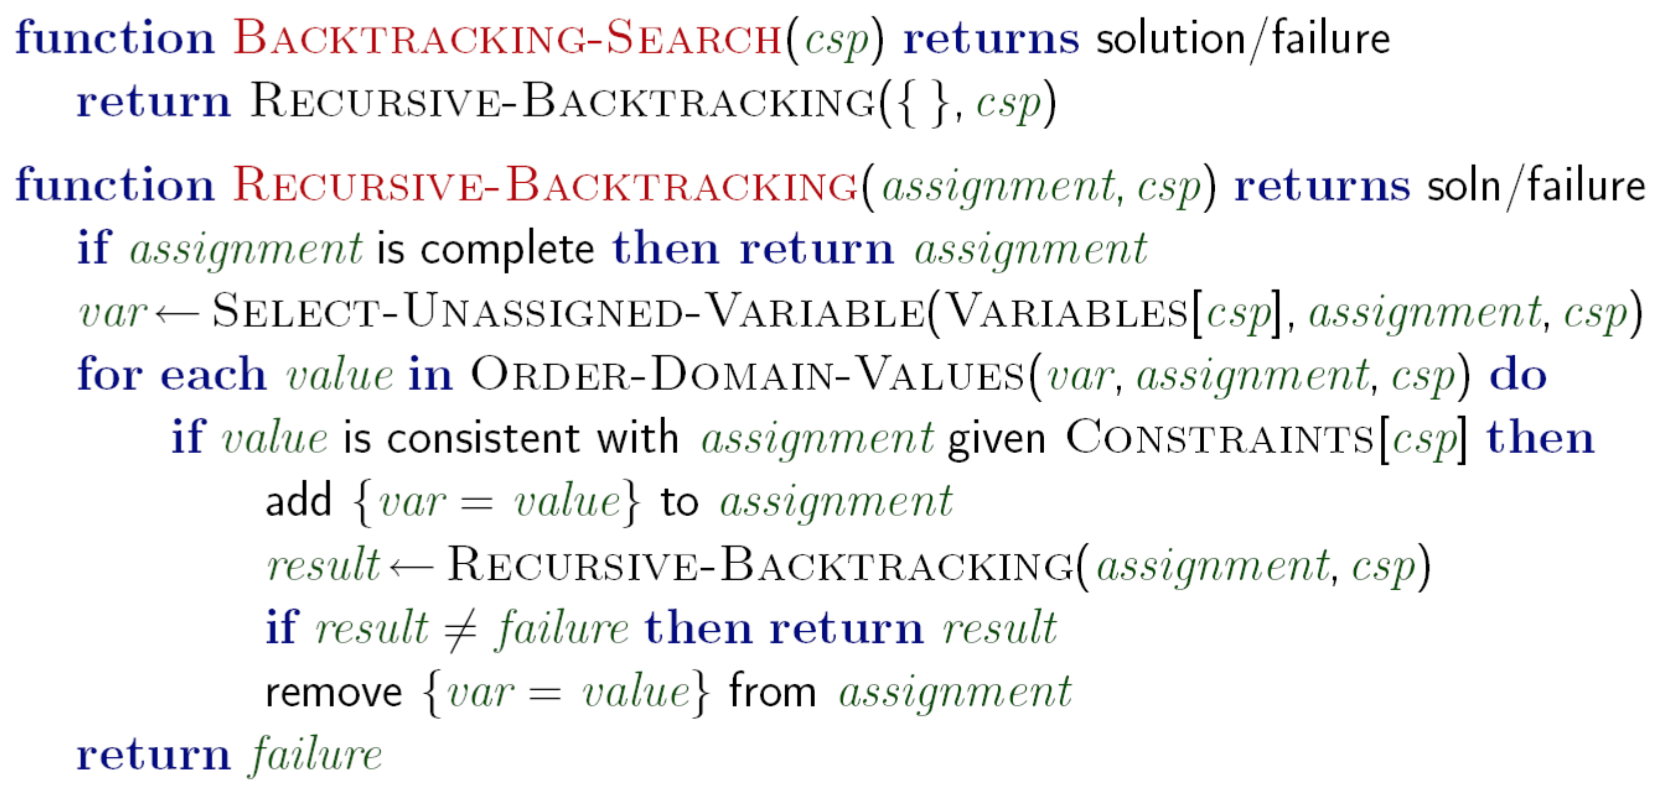
\includegraphics[scale=0.28]{backtracking.png}
        \end{align*}
        \textbf{Optimizations to Backtracking Search:} 
        \item \textbf{Filtering:} 
        \begin{enumerate}
            \item \textbf{Forward Checking:} After a value is assigned to $X_i$, prune the domains of unassigned variables that share a constraint with $X_i$ that would violate the constraint if assigned. In this way, we return failures earlier, when a variable runs out of possible values. But it doesn't provide early detection for all failures.
            \item \textbf{Arc Consistency:} An arc $X \rightarrow Y$ is consistent iff for every $x$ (possible value) in $X$ there is some $y$ (possible value) in $Y$ which could be assigned without violating a constraint. If not for some $x$, delete $x$ from $X$ (the tail). Then re-enqueue all arcs ending at $X$ that had already been dequeued. We run the following algorithm after every assignment:
            \begin{align*}
                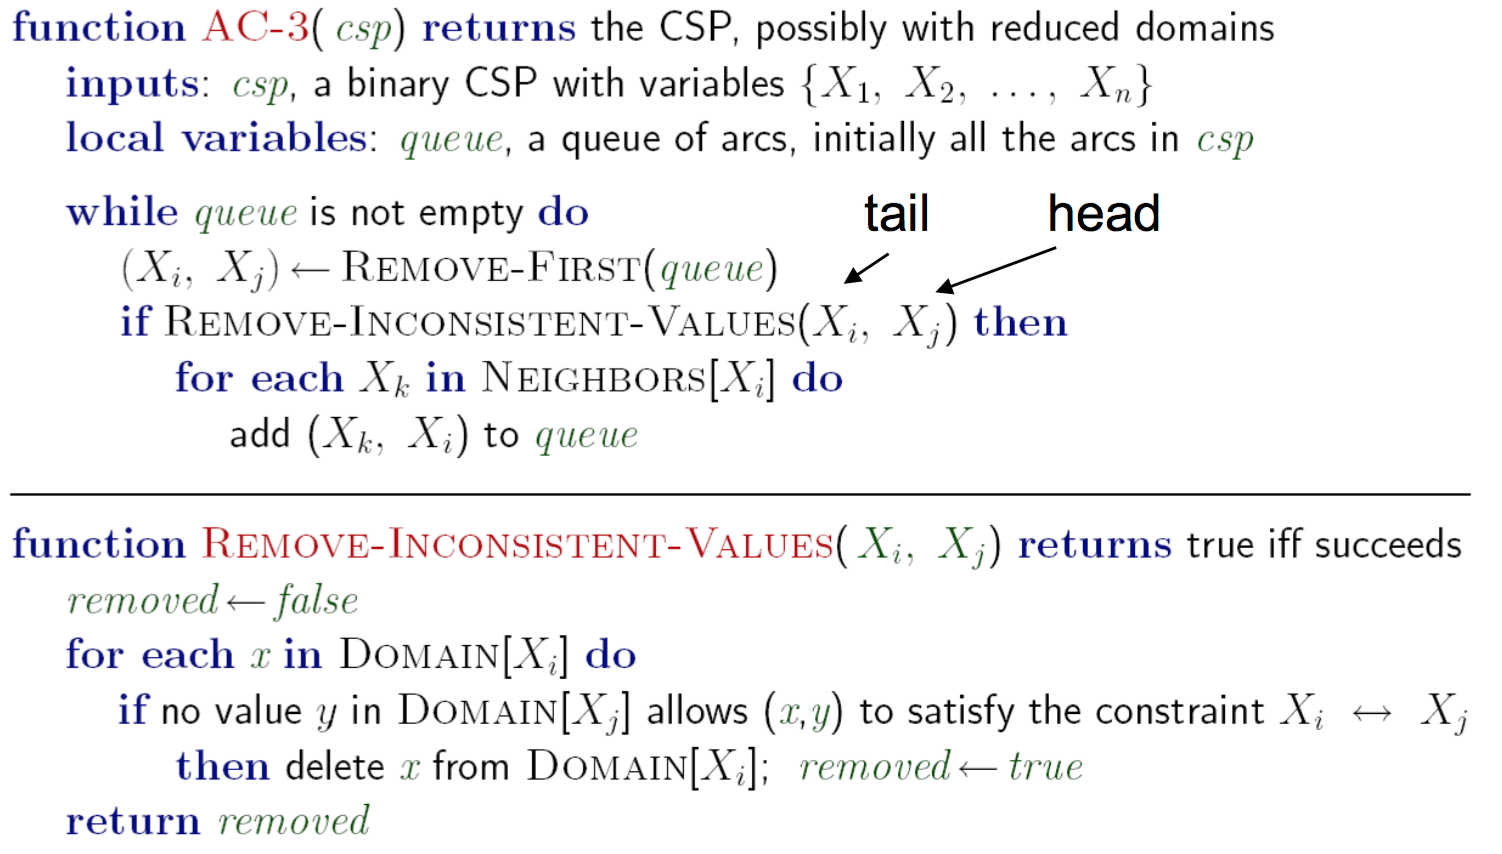
\includegraphics[scale=0.28]{ac.png}
            \end{align*}
            AC-3 is a stronger version of forward checking and finds failure earlier. There are $n^2$ arcs (where $n$ is the number of variables) which each require a $d^2$ checking operation (where $d$ is the size of the domain). Each arc can be put back on the queue at most $d$ times, so run time $O(n^2d^3)$. \\ After enforcing arc consistency, there can be one solution left, many solutions left, or no solutions left (and not know it).
            \item \textbf{$k$-consistency:} For each $k$ nodes, any consistent assignment to $k-1$ can be extended to the $k^{th}$ node. (Arc consistency is 2-consistency). Higher quality filtering, but very costly.
        \end{enumerate}
        \item \textbf{Ordering:} 
        \begin{enumerate}
            \item \textbf{MRV:} Select the variable with the minimum remaining values in its domain next. This is "fail-fast" ordering.
            \item \textbf{LCV:} After picking a variable, order values by least constraining value (that is, from highest total number of values remaining across all variables, to lowest). Requires arc consistency checking.
        \end{enumerate}
        
        \item \textbf{Structure:}
        \begin{enumerate}
            \item A general CSP worst case run time is $O(d^n)$. But if the constraint graph has no loops (i.e., it is a tree), then the CSP can be solved in $O(nd^2)$ time.
            \item The algorithm for a \textbf{tree-structured CSP} is as follows: Choose any variable to be the root variable and order variables so that parents precede children. We remove backward (starting with the right-most node, enforce arc-consistency for the arc from the parent to the node, then do the same for the second-to-right-most node and its parent, and so on). Then we assign forward (start at the left-most node picking any value remaining in its domain, then go to the next variable picking any value in its domain that is consistent with its parent, and continue left to right). We can then find the solution without backtracking in one pass.
            \begin{align*}
                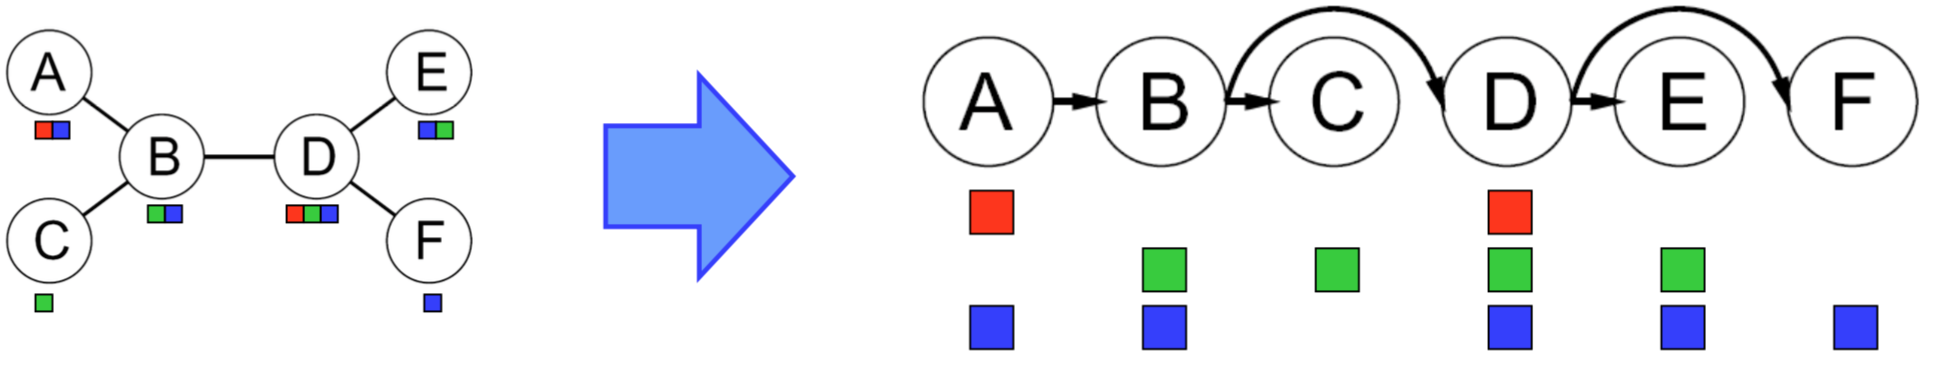
\includegraphics[scale=0.21]{dia.png}
            \end{align*}
             
            \item For nearly tree-structured CSPs, we can use cutset conditioning.
            \begin{align*}
                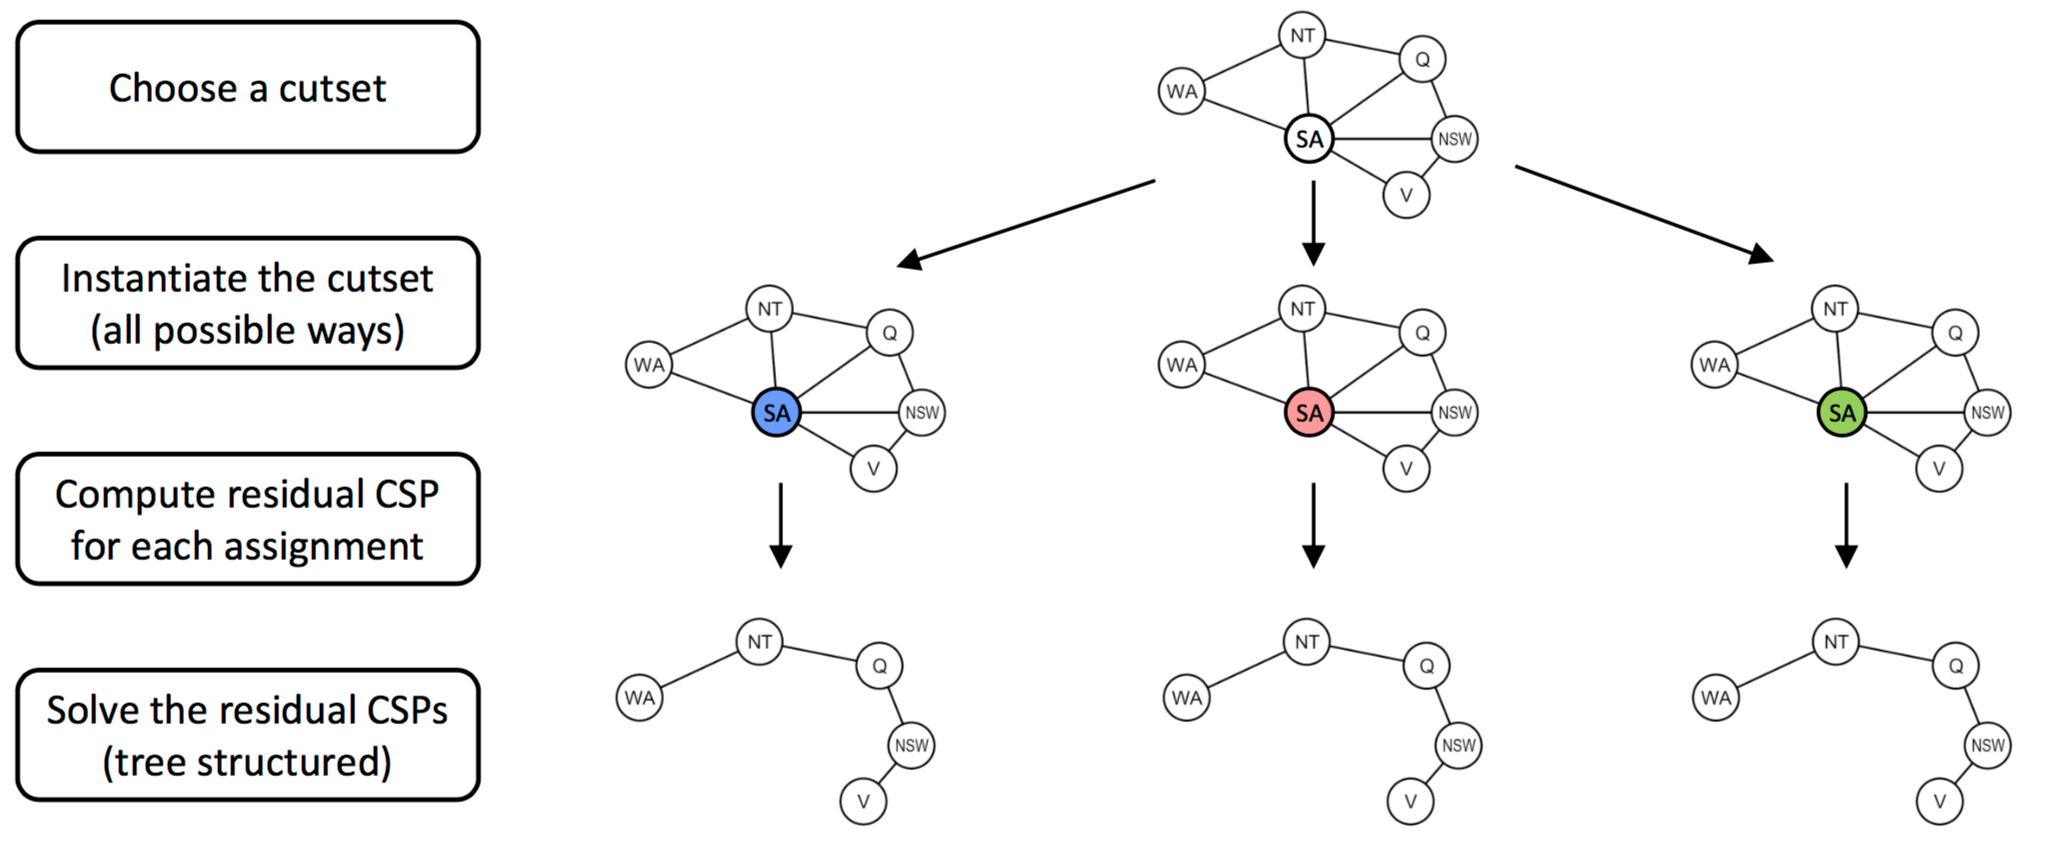
\includegraphics[scale=0.22]{cutset.png}
            \end{align*}
            First find a cutset (i.e. a set of variables such that if removed, the remaining constraint graph forms a tree), then loop over all instantiations of the cutset variables, and for each instantiation call the tree-structured CSP solver to verify if for that instantiation a solution exists. A cutset of size $c$ gives runtime $O(d^c(n-c)d^2)$.
        \end{enumerate}
        \textbf{Iterative Improvement}
        \item Take an assignment with unsatisfied constraints. While not solved, randomly select any conflicted variable and choose a value that violates the fewest constraints.
        \item This simple strategy (called min-conflicts) is often effective in practice. Can solve $n$-queens in almost constant time for arbitrary $n$.
        \item Min-conflicts is an example of local search (as opposed to tree search) because there is no fringe of unexplored alternatives, but only one option that is continuously made better. Faster and more memory efficient, but not complete or optimal.
        \item Another local search is hill climbing: starting anywhere, repeatedly move to the best neighboring state until no neighbors are better than current. The problem is that it may get stuck in a local maximum. 
        \item Can use simulated annealing where we allow downhill moves when no neighbors are better than current, but make them rarer as time goes on. If we decrease the "temperature" slowly enough, we are guaranteed to converge to optimal solution.
        \item Other strategies include random restarts, and genetic algorithms, which are batshit crazy.

    \end{enumerate}
    
    \subsection{Adverserial Search}
    \begin{enumerate}
        \item Adversarial search returns a strategy, or \textbf{policy}, (as opposed to a plan) which simply recommends the best possible move given some configuration.
        \item General games involve agents with independent utilities (values placed on outcomes), while \textbf{zero-sum games} involve agents with opposite utilities where one agent acts to maximize while the other acts to minimize.
        \item A \textbf{game tree} is a directed graph whose nodes are positions in a game and whose edges are actions. The levels, or \textbf{plies}, of a game tree alternate between players. 
        \item A state’s value is defined as the best possible outcome (utility) an agent can achieve from that state. Only terminal state values are known. In adverserial game trees, the \textbf{minimax} value of a node is the best achievable utility against an optimal adversary. If the opponent plays suboptimally, you are guaranteed a better value than minimax. This value is computed mutually recursively: the value of a max agent node is the max of the values of the min agent child nodes, and vice-versa. Same space and time complexity as DFS. 
        \item Complete game trees are realistically impossible to search, so we forget optimality and replace terminal utilities with an evaluation function at a given depth. Such functions are typically weighted linear sums of features.
        
        \textbf{Alpha Beta Pruning:} 
         \item An efficiency improvement to the minimax algorithm that maintains two values, $\alpha$ and $\beta$, which represent the maximum and minimum score that the maximizing agent and minimizing agent is assured of, respectively. Initially $\alpha = - \infty$ and $\beta = \infty$. It can happen that when choosing a certain branch of a certain node, ($\beta \leq \alpha$). If this is the case, the parent node will not choose this node so the other branches of the node do not have to be explored.
        \begin{verbatim}
def value(state, a=MinInt, b=MaxInt):
    if state.isTerminal():
        return state.score
    elif state.agent.isMaxAgent():
        return maxValue(state, a, b)
    else:
        return minValue(state, a, b)

def maxValue(state, a, b):
    v = MinInt
    for successor in state.getSuccessors():
        v = max(v, value(successor, a, b))
        if v >= b:
            return v
        a = max(a, v)
    return v

def minValue(state, a, b):
    v = MaxInt
    for successor in state.getSuccessors():
        v = min(v, value(successor, a, b))
        if v <= a:
            return v
        b = min(b, v)
    return v
        \end{verbatim}
         \item Although intermediate values may be wrong, the pruning has no effect on minimax value computed for the root. This improvement reduces the minimax algorithm's runtime to $O(b^{d/2})$ (when the ordering of child nodes is optimal), effectively doubling the depth the search can go to with the same amount of computation. Optimal ordering is achieved when the best move for a particular agent is it's first child. \\[8 pt]
         \textbf{Expectimax:}
         \item In the traditional \textbf{minimax} algorithm, the levels of the game tree alternate from max to min until the depth limit of the tree has been reached. In an \textbf{expectimax} tree, the "chance" nodes are interleaved with the max and min nodes. Instead of taking the max or min of the utility values of their children, chance nodes take a weighted average, with the weight being the probability that that child is reached. These nodes can represent randomness like dice rolls, or an agent that chooses actions randomly. Thus, the utility at a node under expectimax is always at least as high as the utility of the same node under minimax.
         \item Pruning is not possible with expectimax, since there are no guarantees with node values.
         \item There’s room for robust variation in node layering, allowing for game trees that are modified expectimax/minimax hybrids for any zero-sum game.
         \item Non-zero sum games may involve involve multiple maximixing agents, each trying to maximize their component of a utility tuple. Can give rise to competition or cooperation dynamically.
    \end{enumerate}
    \subsection{Utility}
    \begin{enumerate}
        \item \textbf{Utilities} are functions that take in outcomes and return scores that reflect the preferences of the agent. The principle of maximum expected utility is that a \textit{rational} agent should chose the action that maximizes its expected utility, given its knowledge. In artificial intelligence, we hard-wire utilities to let behaviors emerge.
        \item For the minimax algorithm, the scale of the evaluation function doesn't matter: only the ordering of the children matters. States are insensitive to \textit{monotonic transformations}, or any transformation that preserves ordering (such as squaring).
        \item In contrast, for expectimax, the magnitude of a state must be meaningful, so states are sensitive to monotonic transformations.
        \item An agent must have preferences among prizes $A, B,\hdots$ and lotteries $L=[p,A;(1-p)B]$. 
        \begin{itemize}
            \item Preference: $A \succ B$
            \item Indifference: $A \sim B$
            \item Prefers or indifferent to: $A \succeq B$
        \end{itemize}
        \item There exist constraints on preferences to be considered rational. Rational preferences imply behavior describable as maximization of expected utility. The axioms of rationality:
        \begin{enumerate}
            \item $(A \succ B) \lor (B \succ A) \lor (A \sim B)$
            \item $(A \succ B) \land (B \succ C) \implies (A \succ C)$
            \item $A \succ B \succ C \implies \exists p$ $[p,A;1-p,C] \sim B$
            \item $A \sim B \implies [p,A;$ $1-p,C] \sim [p,B;$ $1-p,C]$
            \item $A \succ B \implies (p \geq q \iff [p,A;$ $1-p,B] \succeq [q,A;$ $1-q,B]$
        \end{enumerate}
        \item The principle of MEU says that for any rational preferences, there exists a real-valued function $U$ consistent with these preferences such that 
        \begin{itemize}
            \item $U(A) \geq U(B) \iff A \succeq B$ 
            \item $U([p_1,S_1;\hdots;p_nS_n]) = \sum_{i}^{}p_iU(S_i)$
        \end{itemize}
        We see that a utility function is risk-seeking if it is concave up; risk-averse if it is concave down; and risk-neutral if the slope is constant.
        
    \end{enumerate}
    
    \subsection{Markov Decision Processes}
    \begin{enumerate}
        \item Now we dive deep into non-deterministic search, which we were introduced to by expectimax. An MDP consists of \begin{enumerate}
            \item Set of \textbf{states} (represented the same as in traditional search problems), including a start state and possibly one or more terminal states.
            \item Set of \textbf{actions}.
            \item A discount factor $\gamma$.
            \item \textbf{Transition function} $T(s,a,s')$ that returns the probability of ending up in $s'$ by taking action $a$ from state $s$.
            \item \textbf{Reward function} $R(s,a,s')$ that returns the reward (positive or negative depending on if it benefits the agent) for ending up in $s'$ by taking action $a$ from state $s$.
        \end{enumerate}
            \begin{align*}
             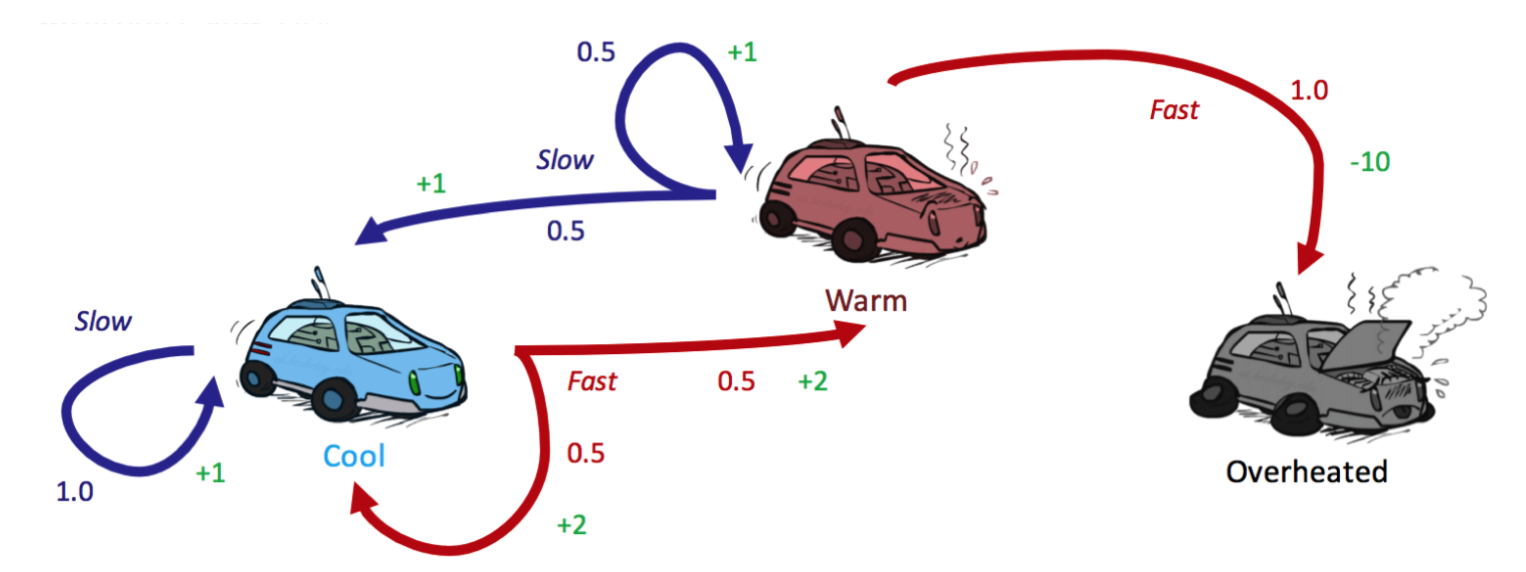
\includegraphics[scale=0.3]{mdp.png}
            \end{align*}
            \item MDPs are "Markovian" in the sense that the probability of arriving in a state $s'$ at time $t + 1$ depends only on the state $s$ and action $a$ taken at time $t$.
            \item Uncertainty in MDPs is modeled by \textbf{q-states}, denoted by the tuple $(s,a)$, which are like expectimax "chance" nodes: they represent an action having been taken but has yet to be resolved into a successor state.
            \item The goal of MDPs is to \textit{maximize utility} (which is the sum of rewards here). To stop MDPs from obtaining infinite reward, we enforce finite horizons or discount factors. \textbf{Finite horizons} gives an agent a fixed number of timesteps to acrue as much reward as possible.
            \item \textbf{Discount factors} model exponential decay of rewards over time. The utility is given by $\sum_{t=0}^{\infty} \gamma^t R(s_t,a_t,s_{t+1})$. When $|\gamma| < 1$, this sum is finite valued, in that it must be $ \leq \frac{R_{max}}{1-\gamma}$. \\[8 pt]
            \textbf{Solving MDPs}
            \item Solving an MDP amounts to finding an optimal policy $\pi^*(s)$, a function that maps each state $s$ to an action that, if taken, will yield the maximum expected utility.
            \item First, we introduce a framework for testing optimality. Denote the optimal value of a state $s$ as $V^*(s)$, which is the expected utility an optimal agent recieves starting from $s$. Denote the optimal value of a q-state $(s,a)$ as $Q^*(s,a)$, which is the expected utility an optimal agent receives starting in $s$ and taking action $a$. \\
            Then, 
            $$V^*(s)=\max_{a}Q^*(s,a)$$ and $$Q^*(s,a)=\sum_{s'} T(s,a,s') [R(s,a,s')+\gamma V^*(s')]$$
            From this, we get the Bellman equation:
            $$V^*(s)=\max_{a}\sum_{s'} T(s,a,s') [R(s,a,s')+\gamma V^*(s')]$$
            We conclude that if we can determine a value $V(s)$ for each state $s$ such that the Bellman equation holds true for each state, then $V(s)=V^*(s)$.
            \item \textbf{Value Iteration} computes optimal values of states. It is a dynamic programming algorithm that uses an iteratively longer time limit to compute time-limited values until convergence. It works as follows:
            \begin{enumerate}
                \item $\forall s$, initialize $V_0(s)=0$.
                \item $\forall s$, repeat until values converge:
                $$V_{k+1}(s) \leftarrow \max_{a}\sum_{s'} T(s,a,s') [R(s,a,s')+\gamma V_k(s')]$$
            \end{enumerate}
            Note that value iteration will actually converge to the same vector of values from \textit{any} intitial values.
            For all $s$, we can interpret the value of $V_{k}(s)$ as the optimal value of $s$ with a time limit of $k$ time steps. It is exactly what a depth $k$ expectimax search returns. The runtime of this algorithm is $O(S^2A)$ for each iteration where $S$ and $A$ are the number of states and actions, respectively. For an MDP terminating after $k$ timesteps, expectimax will be $O((SA)^k)$ while value iteration will be $O(SA^2k)$.
            \item \textbf{Policy extraction} allows us to extract the optimal policy once optimal values for states have been found. It is, $\forall s$:
            \begin{align*}
\pi^*(s)&=\argmax_{a} Q^*(s,a) \\ &=\argmax_a \sum_{s'} T(s,a,s') [R(s,a,s')+\gamma V^*(s')]
            \end{align*}
        
            Clearly, it’s better for policy extraction to have the optimal q-values of states. Storing only each $V^*(s)$ means that we must recompute all necessary q-values with the Bellman equation, equivalent to performing a depth-1 expectimax.
            \item \textbf{Policy Iteration} uses iterative convergence to compute an optimal policy. It tends to outperform value iteration, by virtue of the fact that policies usually converge must faster than the values of states. It works as follows:
            \begin{enumerate}
                \item Define an arbitrary initial policy $\pi_0(s)$; that is, fix a single action for each state.
                \item Evaluate the current policy with \textbf{policy evaluation}: for a policy $\pi$, compute $V^\pi(s)$ for all $s$, where $V^\pi(s)$ is the expected utility received starting in $s$ following policy $\pi$: $$V^\pi(s)=\sum_{s'} T(s,\pi(s),s') [R(s,\pi(s),s')+\gamma V^\pi(s')]$$
                Note that without the max operator, this becomes a linear system of $S$ equations that we can solve. We could also just use the update rule as in value iteration, but this is slower (runtime is $O(S^2)$ for each update).
                \item Use \textbf{policy improvement} to generate a better policy. It runs policy extraction on the (non-optimal!) values obtained from the policy evaluation. $\forall s$,
                $$\pi_{i+1}(s)=\argmax_{a} \sum_{s'} T(s,a,s') [R(s,a,s')+\gamma V^{\pi_i}(s')]$$
                \item Repeat (ii) and (iii) until $\pi_{i+1}=\pi$, at which point the policy has converged and we conclude we have reached $\pi^*(s)$.
            \end{enumerate}
        \item Both value iteration and policy iteration are guaranteed to converge for any finite MDP with discount factor $0 < \gamma < 1$.
    \end{enumerate}
    
    \subsection{Reinforcement Learning}
    \begin{enumerate}
        \item We previously solved MDPs through offline planning; agents had full knowledge of transition and reward functions, so it was possible to precompute optimal actions without ever taking actions.
        \item In online planning, an agent must explore and receive feedback, which it uses to estimate an optimal policy before using this policy for exploitation (reward maximization). This is called \textbf{reinforcement learning.}
        \item At each timestep in online planning, an agent starts in $s$, takes action $a$, ends up in $s'$, and recieved a reward $r$. The tuple $(s,a,s',r)$ is a \textbf{sample}; a string of samples is an \textbf{episode.} \\[8 pt]
        \textbf{Model-Based Learning} 
        \item An agent generates an approximation of the transition function $\Est{T}(s,a,s')$ by normalizing the counts it has collected: divide the count for $(s,a,s')$ by the count for $(s,a)$. Whenever we see fit, we can end the agent's training and switch to exploitation by running value or policy iteration on the obtained $\Est{T}$ and $\Est{R}$ values. 
        \item The idea is simple but the memory overhead can be costly. \\[8 pt]
        \textbf{Model-Free Learning}
        \item Direct evaluation and temporal difference learning are examples of \textbf{passive reinforcement learning}, in which an agent does policy evaluation. (We cannot approximate optimal values directly because the max operator doesn't allow for weighted averaging). Q-learning is an example of \textbf{active reinforcement learning}, in which an agent iteratively updates its policy while learning until determining the optimal policy.
        \item \textbf{Direct evaluation} fixes some policy $\pi$ and has the agent experience several episodes, keeping count of total utility gained \textit{starting from} each state in the episode, and the number times it visited each state. It computes the estimated value of any state $s$ by dividing the total utility obtained from all episodes involving $s$ by the number of times $s$ was visited. This method is unnecessarily slow to converge.
        \item \textbf{Temporal difference learning} uses the idea of learning from every experience, rather than just at the end of an episode. We initialize all states $s$ to $V^{\pi}(s)=0$. At each timestep, an agent takes $\pi(s)$ to get to $s'$ and receives $R(s,\pi(s),s')$. We obtain a \textbf{sample value}: 
        $$\textit{sample}=R(s,\pi(s),s')+\gamma V^{\pi}(s')$$ and incorporate into the existing model for $V^{\pi}(s)$ with an \textbf{exponential moving average}: $$V^{\pi}(s) \leftarrow (1-\alpha)V^{\pi}(s)+\alpha \cdot \textit{sample}$$
        where $\alpha$ is the \textbf{learning rate}. It's typical to start out with $\alpha=1$ and slowly shrink it towards 0. The model for $V^{\pi}(s)$ only improves, so we see that older (thus less accurate) samples are given exponentially less weight. This method learns at every timestep, and converges to true state values much faster with fewer episodes than direct evaluation.
        \item \textbf{Q-learning} learns the q-values of states directly. It approximates \textbf{q-value iteration}, which obeys the following update rule:
        $$Q_{k+1}(s,a) \leftarrow \sum_{s'} T(s,a,s')[R(s,a,s')+\gamma \max_{a'}Q_k(s',a')]$$
        Q-learning acquires q-value samples at every transition:
        $$\textit{sample}=R(s,a,s')+\gamma\max_{a'} Q(s',a')$$ and incorporates them into an exponential moving average:
        $$Q(s,a) \leftarrow (1-\alpha)Q(s,a)+\alpha \cdot \textit{sample}$$ 
        These updates mimic Bellman updates eventually. Whereas TD learning and direct evaluation learned the values of states under a specific policy, Q-learning learns optimal q-values for every state even when taking suboptimal actions.
        \item To ensure convergence, $\alpha$ must be decreased to 0 over time. In RL, we cannot \textit{guarantee} optimal value convergence unless we allow for infinite exploration. \\[8 pt]
        \textbf{Approximate Q-learning}
        \item Q-learning isn't practically efficient when we must store data for millions of q-states. Approximate Q-learning learns about general experiences and extrapolates to many similar situations. The key is to represent states (and q-states) as \textbf{feature vectors} which encode important properties of the state, such as distance to closest pellet, distance to closest ghost, number of ghosts, etc. Then we can write state or q-state values as linear value functions:
        \begin{align*}
            V(s)&=\vec{w} \cdot \vec{f}(s) \\
            Q(s,a)&= \vec{w} \cdot \vec{f}(s,a)
        \end{align*}
        where $\vec{w}=\begin{bmatrix} w_1 & w_2 & \hdots & w_n \end{bmatrix}$ are weights and $\vec{f}(s,a)=\begin{bmatrix} f_1(s,a) & f_2(s,a) & \hdots & f_n(s,a) \end{bmatrix}^T$ are the features. Approximate Q-learning recieves a sample and computes a difference: $$\textit{difference}= [R(s,a,s')+\gamma\max_{a'} Q(s',a')] - Q(s,a)$$ then performs the following update: 
        \begin{align*}
            Q(s,a) &\leftarrow Q(s,a) + \alpha \cdot \textit{difference} \\
            w_i &\leftarrow w_i + \alpha \cdot \textit{difference} \cdot f_i(s,a)
        \end{align*}
        Thus, we adjust the weight of the active features according to how large a role they played in an incorrect model prediction. \\[8 pt]
        \textbf{Exploration vs Exploitation}
        \item Agents following an \textbf{$\epsilon$-greedy} policy define some probability $0 \leq \epsilon \leq 1$ and explore randomly with probability $\epsilon$ and exploit with probability $(1-\epsilon)$. To find a balance is tricky, and requires fine-tuning.
        \item \textbf{Exploration functions} eliminate the need for manually setting exploration time. Agents choose actions given by an exploration function, which often takes the form $$f(s,a)=Q(s,a)+\frac{k}{N(s,a)}$$ where $N(s,a)$ denotes the number of times $(s,a)$ has been visited, and $k$ is some fixed amount. Exploration is automatically encoded by the exploration function, since the term $\frac{k}{N(s,a)}$ gives a bonus to infrequently taken actions. It uses a modified q-value update:
        $$Q(s,a) \leftarrow (1-\alpha)Q(s,a)+\alpha[R(s,a,s')+\max_{a'}f(s',a')]$$
        As time goes on, this bonus decreases to 0, so $f(s,a)$ regresses to $Q(s,a)$ and we are back to regular q-learning.
        \end{enumerate}
    \end{enumerate}
    \section{Probabilistic Inference}
    \begin{enumerate}
        \subsection{Probability}
        \begin{enumerate}
            \item \textbf{Random variables}, denoted by capital letters, represent aspects of the world that are uncertain. For random variables with binary domains, we sometimes say $\{+x, -x\}$.
            \item A \textbf{probability distribution} is a table of value, probability pairs for each value a random variable can take on, such that the sum of the probabilities is 1.
            \item A \textbf{joint distribution} over a set of random variables $X_1, X_2, \hdots, X_n$ specifies a probability to each assignment $P(x_1, x_2, \hdots, x_n)$ for each $x_i \in X_i$ such that the sum of the probabilities is 1.
            \item An event is a set of full or partial assignments, so rows in a joint distribution. 
            \item Marginal distributions are sub-tables which eliminate variables; \textbf{marginalization} is the process of summing over a variable to eliminate it. 
            \item Conditional probability:
            $$P(a|b) = \frac{P(a,b)}{P(b)}$$
            \item A \textbf{conditional distribution} is a probability distribution over some variables given fixed values of others. Can be obtained from a joint distribution by selecting the assignments that match the evidence and normalizing (dividing every entry by sum over entries) the selection.
            \item \textbf{Inference by enumeration:} We have a set of evidence variables (variables for which we know the values of), a query variable, and hidden (unknown) variables. First we select all entries consistent with the evidence. Then we sum out hidden variables to get a joint distribution with only the query and evidence variables. Lastly normalize.
            \item \textbf{Chain rule:} We can write any joint distribution as a product of conditional distributions:
            $$P(x_1, \ldots, x_n) = \prod_{i=1}^{n} P(x_i | x_{i-1}, \ldots, x_1)$$
            \item \textbf{Bayes' Rule:} $$P(a|b) = \frac{P(b|a)P(a)}{P(b)}$$
            \item Two variables $X$ and $Y$ are \textbf{independent} ($X \upmodels Y$) iff  $\forall x, y$ $P(x,y)=P(x)P(y)$, or equivalently $P(x|y)=P(x)$. Given a joint distribution, we can test for independence by marginalizing, then seeing if the joint distribution formed as if $X$ and $Y$ were independent is the same as the original joint distribution.
            \item Two variables $X$ and $Y$ are \textbf{conditionally independent} given $Z$ ($X \upmodels Y | Z$ and $Y \upmodels X | Z$) iff $\forall x,y,z$ $P(x,y|z)=P(x|z)P(y|z)$ or equivalently $P(x|y,z)=P(x|z)$. Conditional independence allows us to simplify terms in the chain rule product for a joint distribution. 
             
        \end{enumerate}
    \subsection{Bayes' Nets}
    \begin{enumerate}
        \item Bayes' Nets are a technique of implicitly encoding complex joint distributions as simple local interactions. We can perform probabilistic inference using them. They are directed, acyclic graphs with variables as nodes and edges indicating direct influence between variables.
        \item To recover the probability of an assignment:
        $$P(x_1,\ldots,x_n) = \prod_{i=1}^{n}P(x_i | \textit{parents} (X_i))$$
        \item Bayes' Nets need not reflect causal patterns. The fewer the arrows, the more conditional independence assumptions; it is only mandatory that a Bayes Net does not make \textit{additional} independence assumptions.
        \begin{align*}
            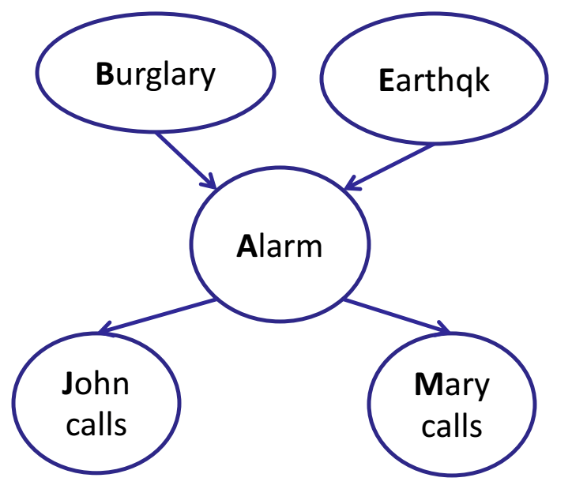
\includegraphics[scale=0.2]{bn.png}
        \end{align*}
        \item \textbf{Reasoning about Independence} \\
        We know each variable is conditionally independent of its non-descendants, given its parents. We can go further with d-separation: Given a particular query, ask a question about the independence of two variables. For example, for the query $P(A|B)$ we ask "are A and B independent"?, or for the query $P(A|B,C,D)$ we ask "are A and B conditionally independent given C and D"?
        \begin{enumerate}
            \item Draw the ancestral graph (i.e., the graph of only the variables in question and their ancestors- parents, parent's parents, etc).
            \item For every pair of variables with a common child in the ancestral graph, draw an undirected edge between them.
            \item Replace all directed edges with undirected edges.
            \item Delete the given variables (if any) and their edges. Then: 
        \end{enumerate}
        \begin{itemize}
            \item If the variables are disconnected (a path does not exist, or one or both variables were removed because they were given) in this graph, they are guaranteed to be independent.
            \item If the variables are connected in this graph, they are not guaranteed to be independent.
        \end{itemize} 
        \item Probabilistic inference, or calculating some useful quantity from a joint distribution, is NP-complete. Enumeration is exact but exponential complexity. Variable elimination is exact with worst-case exponential complexity. Sampling is approximate.
        \item \textbf{Inference by enumeration} in Bayes' Nets, following the same setup as described earlier, works as follows: 
        \begin{enumerate}
            \item We track objects called factors. Initial factors are the conditional probability tables encoded by each node, with only the rows of known values (if there any).
            \item Join all factors. That is, for each variable, join all factors with that variable by point-wise multiplication. In a join operation, the unconditioned variables in the resulting CPT consist of the \textit{set} of input unconditioned variables, and the conditioned variables in the resulting CPT consist of all input variables not in the unconditioned set. Finally  join all remaining factors. Ex: To join $P(R)$ and $P(T|R)$, each entry in $P(R,T)$ is $P(r,t)=P(r)P(t|r)$, $\forall r,t$.
            \item Now we have the full relevant joint distribution. Marginalize each hidden variable by summing it out to shrink the factor. Lastly normalize.
        \end{enumerate}
        \item \textbf{Variable elimination} interleaves joining and marginalizing, which is usually much faster. It works by starting off with initial factors (instantiated by evidence), then while there are hidden variables: pick a hidden variable $H$, join all factors with $H$, then sum out $H$. Join all remaining factors and normalize.
        \item The computational complexity depends on the size (number of entries) in the largest factor. The order of variables to eliminate greatly affects this size; there does not always exist an order that produces small factors. In general, it is best to choose variables that appear in the fewest number of CPTs first.
        \item \textbf{Sampling} is faster than variable elimination, and eventually converges to the true probability.
        \begin{enumerate}
            \item \textbf{Prior sampling:} A sample of a full assignment is obtained as follows: for each variable in the Bayes' Net in topological order, draw a random value from [0, 1). Map this value to the corresponding assignment from the variable's CPT given any previous assignments. Add this variable's assignment to the list of assignments. Once every variable has been assigned, the sample is complete.
        \end{enumerate}
        We can answer queries from samples by computing the number of samples consistent with the query divided by the number of samples consistent with evidence (if any). \\
        If we know the query in advance, we can sample more efficiently:
        \begin{enumerate}
            \item \textbf{Rejection sampling} stops computing a sample once an evidence variable has been assigned a value inconsistent with the query evidence. This method can still be inefficient when evidence variables are "downstream", or the evidence is unlikely.
            \item \textbf{Likelihood weighting} solves these problems by forcing evidence variables to be consistent with the query. Each sample must also have a corresponding weight, which is the product of the probabilities of the evidence variables taking on their forced values given the other assignments. Then, to answer queries, we instead compute the sum of the weights of samples consistent with the query divided by the sum of the weights of samples consistent with the evidence.
        \end{enumerate}
        Weights obtained by likelihood weighting can be very small if upstream variables (before evidence) are unlikely given the evidence, making samples less useful. 
        \begin{enumerate}
            \item \textbf{Gibbs sampling} effectively samples \textit{all} variables conditioned on evidence. It works as follows: first generate an arbitrary sample consistent with evidence. To generate a new sample, choose a non-evidence variable $X$ and resample $X$ given all other assignments (can be done efficiently, as only CPTs with resampled variable need be considered). Repeating this infinitely many times yields samples with correct distribution. 
        \end{enumerate}
    \end{enumerate}
    
    \subsection{Decision Networks and VPI} 
    \begin{enumerate}
        \item Decision networks are generalizations of Bayes' Nets that allow us to choose actions which maximize expected utility given evidence. 
        \begin{align*}
            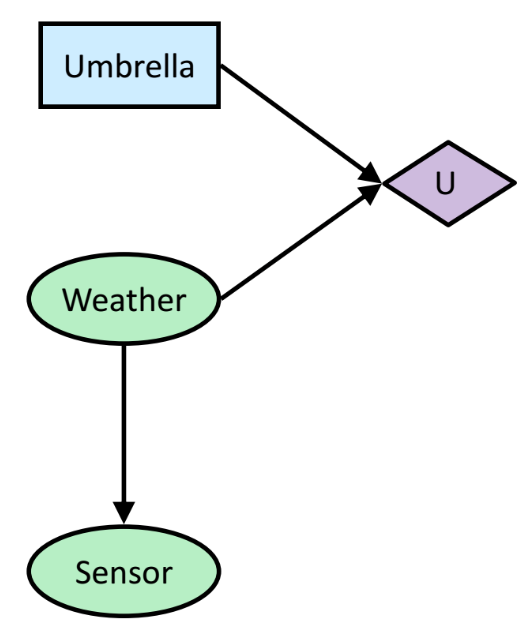
\includegraphics[scale=0.2]{dn.png}
        \end{align*}
        \item In addition to random variable nodes, there are also action nodes (rectangles) that represent decisions and cannot have parents, and utility nodes (diamonds) which give the utility of each possible action and variable value.
        \item To select an action, we instantiate all evidence. Then calculate the posterior probability (probability given the evidence) of all parents of utility node. Then calculate the expected utility for every action, and choose action with MEU.
        \item The \textbf{value of perfect information} is the \textit{expected} gain in MEU if we knew the value of a variable:
        $$\textit{VPI}(E'|e)=\left( \sum_{e' \in E'} P(e'|e)\textit{MEU}(e,e') \right) - \textit{MEU}(e)$$
        where $E$ is a random variable and \textit{MEU} is a function of evidence:
        $$\textit{MEU}(e)=\max_{a}\textit{EU}(a)$$
        In other words, \textit{VPI(E)} represents the utility we we'd be willing to spend to get perfect information about $E$.
        \item VPI is always 
        \begin{enumerate}
            \item non-negative
            \item zero for any node that is conditionally independent given the evidence so far of all parents of the utility node
            \item non-additive; sometimes knowing the value of one variable lessens the value of knowing another variable
            \item order-independent: 
            \begin{align*}
     \textit{VPI}(A,B)&=\textit{VPI}(A)+\textit{VPI}(A|B) \\ &= \textit{VPI}(B)+\textit{VPI}(B|A)
            \end{align*}
        \end{enumerate}
    \end{enumerate}
    \subsection{Hidden Markov Models}
    \begin{enumerate}
        \item \textbf{Markov models} specify how a state $X$ changes over time. The past is conditionally independent of the future given the present. Note that we have encountered these before in the context of MDP transitions; however, here there will not be choice of action.
        \item The only parameter is $P(X_t | X_{t-1})$, or the transition probabilities. The distribution at timestep infinity $P_{\infty}(X)$ is independent of the initial distribution and is called the \textit{stationary distribution}. This is the idea behind Google's pagerank.
        \item A \textbf{hidden Markov model} is a Markov chain for which the state is only partially observable; at each timestep, we observe the effects of the underlying Markov chain. Ex: in speech recognition, acoustic signals are observations, specific words are states.
        \begin{align*}
            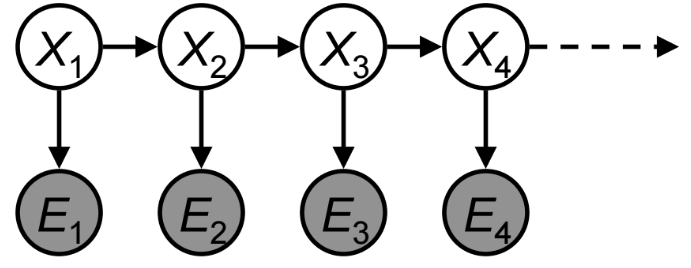
\includegraphics[scale=0.2]{hmm.png}
        \end{align*}
        An HMM is defined by transitions $P(X_t | X_{t-1})$, an initial distribution $P(X_1)$, and emissions $P(E_t | X_t)$. 
        \item An HMM is the simplest \textbf{Dynamic Bayes' Net}, or a Bayesian network which relates variables to each other over adjacent time steps.
        \item \textit{Filtering} or \textit{monitoring} is the task of tracking the belief distribution $B_t(X)=P(X_t | e_1, \ldots, e_t)$, i.e., the belief in the distribution of $X$ at time $t$. We start with $B_1(X)$, which is usually uniform, and update as we get observations. \\
        Online belief update, also called the \textbf{forward algorithm}, is a dynamic programming algorithm to solve this:
        \begin{enumerate}
            \item We have $B_t(X)=P(X_t | e_{1 \rightarrow t})$.
            \item One timestep occurs. We have $$B'_{t+1}=P(X_{t+1} | e_{1 \rightarrow t}) = \sum_{x_t} P(X_{t+1} | x_t)B_t(x)$$ (prior beliefs in distribution times transition probabilities).
            \item Evidence comes in. We have $$B_{t+1}=P(X_{t+1} | e_{1 \rightarrow t+1}) \propto_{X_{t+1}} P(e_{t+1} | X_{t+1}) B'_{t+1}(X)$$ (beliefs are reweighted by emissions).
        \end{enumerate}
        \item The \textbf{Viterbi algorithm} is a dynamic programming algorithm that will compute the most-likely explanation, or corresponding sequence of states, given a sequence of observations. Let $m_t(x_t)$ denote the probability of the most likely sequence of states given the evidence. Then $$m_t(x_t) = P(e_t | x_t) \max_{x_{t-1}}P(x_t | x_{t-1})m_{t-1}(x_{t-1})$$
        Return the actual sequence by maintaining pointers. Note that the update is identical to that of the Forward Algorithm, except with a max operator instead of a sum.
        \item \textbf{Particle filtering} is an approximate method to find $B_t(X)$. In practice, the domain of $X$ can be too large to store in memory (such as in robot locationing), so it is more efficient to store a list of samples and their corresponding values of $X$, called particles. Then, $P(X=x)$ is approximated by the number of particles with value $x$.
        \begin{enumerate}
            \item Each particle is moved by sampling its next location from the transition probabilities. 
            \item After observing evidence $e$, assign particles of value $x$ a weight of $P(e|x)$. 
            \item Re-sample particles from the weighted sample distribution; this is equivalent to normalizing the distribution. 
        \end{enumerate}
    \end{enumerate}
\end{enumerate}
\section{Machine Learning}
\begin{enumerate}
    \subsection{Classification with Naive Bayes}
    \begin{enumerate}
        \item For the most part, we have discussed using models to solve problems and make optimal decisions. Machine learning is the process of acquiring models from data. 
        \item Classification is a supervised machine learning task to identify the category to which an input belongs. \textit{Features} are the attributes used to make the decision. For example, in spam filtering, features may include words in text, text patterns, whether the sender is a contact, etc.
        \item A \textbf{Naive Bayes} model is a simple classifier:
         \begin{align*}
             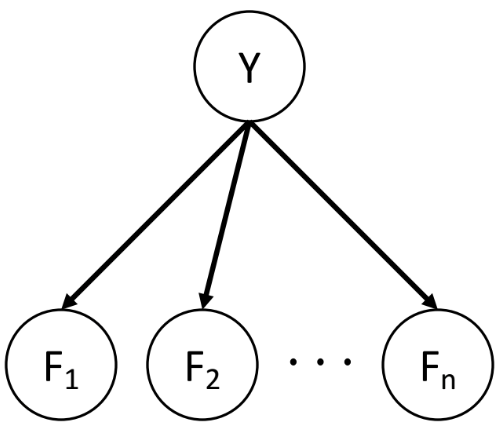
\includegraphics[scale=0.35]{naivebayes.png}
         \end{align*}
        All features are assumed to be independent of all others, given the class. This is unrealistic, but often works well in practice. 
        \item We have $P(Y|F_1,\ldots,F_n) \propto P(Y) \prod_{i=1}^{n} P(F_i|Y)$. There are $n \times |F|\times |Y|$ \textbf{parameters}, which is linear in $n$. The number of parameters is constant in $n$ for spam filtering, since each feature CPT is the same. In contrast, in optical character recognition, $Y$ takes on values in $[0,9]$ and each feature node encodes the probability of a particular pixel being illuminated given the character. A common trick to reduce the number of parameters is to write one parameter as the complement of the sum of other parameters, when possible.
        \item Given the parameters ($P(Y)$ and $P(F_i|Y)$), classificiation is done by computing $P(Y|F_1,\ldots,F_n)$ (or the log) and returning the value of $Y$ with the highest probability. 
        \item Where do we get parameters? \textbf{Maximum likelihood estimation (MLE)} finds the parameter values that maximize the likelihood of the observations given the parameters. That is, we set $$P_{ML}(x) = \frac{\text{count}(x)}{N}$$ For example, MLE in spam filtering would set $P(\text{spam}, w_i=w)$ to the number of times $w$ appears in a spam email divided by the total number of words in all spam emails.
        \item The problem with using relative frequencies for parameters is that of \textit{overfitting}; we cannot assign unseen events 0 probability. To generalize better, we need to \textit{smooth} the estimates. 
        \item In \textbf{Laplace Smoothing}, we pretend we saw each sample $k$ more times. That is, we set
        $$P_{LAP,k}(x) = \frac{\text{count}(x)+k}{N+k|X|}$$
        $k$ is a hyperparameter and can be interpreted as the strength of the prior belief. For conditionals, this is
        $$P_{LAP,k}(x|y) = \frac{\text{count}(x,y)+k}{\text{count}(y)+k|X|}$$
        \item The general process in machine learning involves learning parameters from training data; tuning hyperparameters on hold-out data (i.e., choosing the values that maximize accuracy on hold-out data); then computing accuracy from the test data.
        
    \end{enumerate}
    \subsection{Classification with Perceptrons}
    \begin{enumerate}
        \item A \textbf{Perceptron} is a linear error-driven classifier. Inputs are feature values, and each feature is given a corresponding weight. The activation is the weighted sum: $$\text{activation}_{\vec{w}}=\sum_{i}w_if_i(x)=\vec{w} \cdot \vec{f(x)}$$ 
        If the activation is positive, output +1, otherwise -1 (corresponding to two different classes).
        \item If we want to take into account that one class is inherently more likely, we can create a constant offset by setting the first entry in the weight vector to a bias value, and setting the first entry in the feature vector to be 1 always.
        \item Learning the weights occurs as follows:
        \begin{enumerate}
            \item Initialize $\vec{w}=\vec{0}$.
            \item For each training sample $x$ with feature $\vec{f(x)}$: \\ If correct, no change. Otherwise, if true class was +1, update $\vec{w}_{new} = \vec{w}_{old}+\vec{f}$. If true class was -1, update $\vec{w}_{new} = \vec{w}_{old}-\vec{f}$.
        \end{enumerate}
        \item For multiple classes, simply keep a weight vector for each class and output the class with the highest activation. Learning works the same way, except subtract $\vec{f(x)}$ from wrong answer and add $\vec{f(x)}$ to the right answer. 
        \item \textit{Separability} is the property that there exists some set of parameters to get the training data completely right (i.e., there exists a separating hyperplane). If the training data is linearly separable, then the perceptron \textit{will} eventually converge (binary case); otherwise, it will fail.
        \item The standard update method finds \textit{a} solution (assuming linearly separable data), but not necessarily the optimal solution. \textbf{MIRA} finds the \textit{minimum} correcting update. Suppose we saw sample $x$, predicted it was class $y$, but it was really class $y^*$. Then we want new weight vectors $W$ that minimize the change, but still fix the mistake: 
        \begin{align*}
            \min_{W} \frac{1}{2}\sum_{i} ||\vec{w_i}^{new}-\vec{w_i}^{old}||^2 \\ \textit{s.t.} \hspace{4mm} \vec{w_{y^*}}^{new} \cdot \vec{f(x)} \geq \vec{w_{y}}^{new} \cdot \vec{f(x)} + 1
        \end{align*}
        Note that only two weight vectors in $W$ actually change, namely
        \begin{align*}
            \vec{w_{y^*}}^{new} = \vec{w_{y^*}}^{old} + \tau \vec{f(x)} \\
            \vec{w_{y}}^{new} = \vec{w_{y}}^{old} - \tau \vec{f(x)} 
        \end{align*}
        We find that taking 
        \begin{align*}
            \tau = \frac{(\vec{w_{y}}^{old} - \vec{w_{y^*}}^{old}) \cdot \vec{f(x)}+1}{2\vec{f(x)} \cdot \vec{f(x)}}
        \end{align*}
        satisfies these equations. In practice, we cap the value of $\tau$ with some hyperparameter $C$ to account for noisy data:
        \begin{align*}
            \tau = \min\left( \frac{(\vec{w_{y}}^{old} - \vec{w_{y^*}}^{old}) \cdot \vec{f(x)}+1}{2\vec{f(x)} \cdot \vec{f(x)}}, C \right)
        \end{align*}
        Note that with the original perceptron, the update might not be enough to fix the classification error; hence $\tau$ can be larger or smaller than 1.
        \item \textbf{SVMs} (Support vector machines) find the separator with the maximum margin, which is equivalent to minimizing the magnitudes of the weight vectors. We want to find new weight vectors $W$ of minimum magnitude, but optimize over all samples:
        \begin{align*}
            &\min_{W} \frac{1}{2}\sum_{i} ||\vec{w_i}||^2 \\ \textit{s.t.} \hspace{4mm} \forall i, y: \vec{w_{y^*}} &\cdot \vec{f(x_i)} \geq \vec{w_{y}} \cdot \vec{f(x_i)} + 1
        \end{align*}
        SVMs update weights based on the entire training set (batch), while MIRA updates based on a single training instance at a time (online).
        \item The perceptron algorithm with these modifications, with multiple passes through the data, is often more accurate than the Naive Bayes classifier.
        \item SVMs can perform a non-linear classification by implicitly mapping inputs into high-dimensional feature spaces where they are separable.
    \end{enumerate}
    \subsection{Deep Learning}
    \begin{enumerate}
        \item Manual feature design is difficult, requiring domain-specific expertise. \textbf{Deep learning} is the process of using multilayer \textbf{neural networks} for feature extraction. Each successive layer uses the output from the previous layer as input, forming a hierarchy from low-level to high-level features. 
         \begin{align*}
             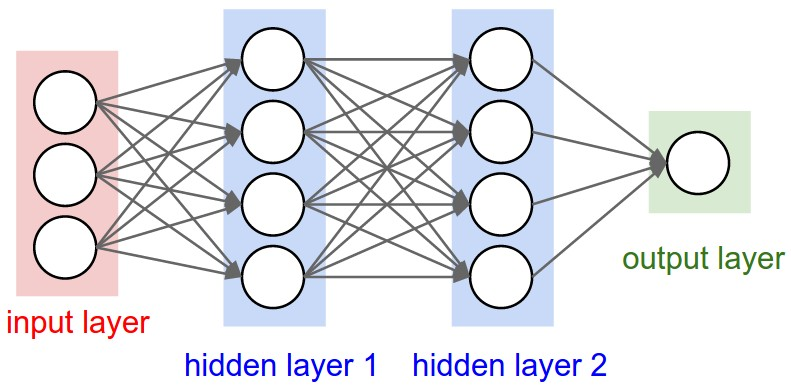
\includegraphics[scale=0.2]{nn.jpg}
         \end{align*}        
        \item The inputs are preliminary features of the data; hidden layers will learn high-level abstractions. The goal is to learn the \textit{weights} of the connections between neurons so as to maximize accuracy on training data.
        \item A \textit{loss function} quantifies the agreement between the predicted labels and the true labels.
        \item The activation function of the linear perceptron (+1 for activation, -1 otherwise) is poor for deep networks, as it is difficult to measure progress and optimize. An example of a nonlinear activation function in deep learning is \textbf{softmax}, where the activation of each class is the probability of the class $y$ being $j$:
        $$ P(y = j | \vec{f(x)}) = \frac{e^{\vec{w_j} \cdot \vec{f(x)}}}{\sum_{i} e^{\vec{w_i} \cdot \vec{f(x)}}}$$
        Note that in the binary case, $\vec{w_1} = - \vec{w_{-1}}$. Softmax is typically used only on the output node due to its normalization denominator. \\ Define the loss function $l(w)$ (of the entire neural network) as follows:
        \begin{align*}
            l(w) = \prod_{i=1}^m P(y = y_i | \vec{f(x_i)})
        \end{align*}
        In training, we wish to learn weights that maximize this function. This is equivalent to maximizing the log of the expression:
        \begin{align*}
            ll(w) = \sum_{i=1}^m \log P(y = y_i | \vec{f(x_i)})
        \end{align*}
        By convention, we minimize $-ll(w)$. This can be done by \textbf{gradient descent}.
        \item Review: If $f(x_1, \ldots, x_n)$ is a differentiable function of several variables, its \textbf{gradient} $\nabla f$ is the \textit{vector} whose components are the $n$ partial derivatives of $f$. In the 3D Cartesian coordinate system, for example, $$\nabla f = \frac{\partial f}{\partial x}\vec{i} + \frac{\partial f}{\partial y}\vec{j} + \frac{\partial f}{\partial z}\vec{k}$$ where $\vec{i},\vec{j},\vec{k}$ are standard unit vectors. 
        \item Gradient descent uses the following weight update in learning:
        $$ w \leftarrow w - \alpha * \nabla g(w) $$ where $g(w) = ll(w)$ and $\alpha$ is the learning rate (which must be carefully chosen and decreased over time). That is, we move weights against the direction of the gradient in order to move to a local minimum in the loss function. There is also sometimes a momentum parameter that adds a fraction of the previous weight update to the current one, which serves to speed up convergence to the minimum by damping oscillations.
        \item Computing the gradient can be done efficiently by finite difference approximation (i.e., applying the limit definition of partial derivatives with small $h$ values). 
        \item Alternatively, Back-propagation is an efficient method that computes the \textit{exact} gradient using the chain rule to iteratively compute gradients at each layer. \\
        A brief overview of how back-propagation on a neural net is performed:
        \begin{enumerate}
            \item We have given inputs (from training data).
            \item Write out the output of the network as a computation graph, naming each connection ($a,b,c,\ldots$) between neurons.
            \item In the forward pass, write the values of each successive computation node (neuron) until reaching the output node $y$. 
            \item In the backward pass, use the expression for the parent node and the chain rule (as well as values of the node) to compute $\frac{\partial y}{\partial c}$ for each connection $c$ until arriving back at the inputs. This yields a gradient vector containing the partial derivative of the output with respect to each weight in the network.
        \end{enumerate}
        \item Random initialization of weights outperforms constant weight initialization, since backpropagation will yield identical gradients for all neurons within each layer, effectively yielding duplicated neurons.
        \item Deep learning is huge field with countless algorithms and variations for certain applications. A few notable optimizations or modifications include:
        \begin{enumerate}
        \item Batch gradient descent involves calculating the gradient on all data (by iterating through and averaging the gradients obtained for each sample). Stochastic gradient descent (which is what we have been discussing) calculates the gradient on one data point only, which is faster but oscilates more depending on the order of samples. Mini-batching involves calculating the gradient for random subsets of data points. This is what's used in practice.
        \item Several activation functions (e.g. $\tanh$, sigmoid, ReLU) are possible, with ReLU ($\max(0,x)$) being the most common choice for intermediate layers.
        \item Larger neural networks always  work better than smaller networks, but they are more prone to overfitting. Dropout is an example of \textit{regularization} that attempts to prevent overfitting. Some number of neurons are randomly omitted with probability $1-p$ from the hidden layers during training in order to break rare dependencies that can occur in training data. The entire neural network is used during test time with outgoing weights scaled by $p$.
        \item \textit{Convolutional Neural Networks} are used in image processing. They consist of multiple layers of receptive fields which process portions of the input image. The outputs of these collections are then tiled so that their input regions overlap. Tiling allows ConvNets to tolerate translation of the input image.
        \end{enumerate}
    \end{enumerate}
\end{enumerate}

\end{multicols}
\end{document}
